% Lecture Template for ME3050 - Dynamic Modeling and Controls - Tennessee Technological University
% Spring 2023 - condensing and streamlining lectures by combining topics into a single PDF under the module name
% this will simplify file and link management as well as make lectures easier to use in class
% - added image/ to clean directory and reduce redundancy, specific to module for now  

% Module Name: - Introduction
% Topic 1 - Components, Units, and Symbols
% Topic 2 - Fundamental Laws
% Topic 3 - Circuit Applications

\documentclass[fleqn]{beamer} % for presentation (has nav buttons at bottom)

%\usepackage{/home/tntech.edu/thill/courses/dmc/lectures/dmc_lectures}
\usepackage{/home/thill/courses/dmc/lectures/dmc_lectures}
%\usepackage{/mnt/c/Users/thill/Documents/courses/dmc/lectures/dmc_lectures}

\author{ME3050 - Dynamics Modeling and Controls}

\newcommand{\MNUM}{1\hspace{2mm}} % module number 
\newcommand{\moduletitle}{Introduction}

\newcommand{\sectionItitle}{System Dynamics}
\newcommand{\sectionIItitle}{Units and Conversions}
\newcommand{\sectionIIItitle}{Models and Assumptions}

\newcommand{\sectionIsubsectionItitle}{Definition of Dynamics}
\newcommand{\sectionIsubsectionIItitle}{Modeling and Analysis}
\newcommand{\sectionIsubsectionIIItitle}{Model Based Design}
\newcommand{\sectionIsubsectionIVtitle}{Course Topics}

\newcommand{\sectionIIsubsectionItitle}{Standard Units}
\newcommand{\sectionIIsubsectionIItitle}{Unit Conversions}
\newcommand{\sectionIIsubsectionIIItitle}{Frequency and Circular Frequency}
\newcommand{\sectionIIsubsectionIVtitle}{Example - Units Matter}

\newcommand{\sectionIIIsubsectionItitle}{Mathematical Modeling}
\newcommand{\sectionIIIsubsectionIItitle}{Solid Mechanics and Dynamics}
\newcommand{\sectionIIIsubsectionIIItitle}{Thermal and Fluid Systems}
\newcommand{\sectionIIIsubsectionIVtitle}{Electrical and Power Systems}

% custom box
\newsavebox{\mybox}

\title{Lecture Module - \moduletitle}

\date{Mechanical Engineering\vspc Tennessee Technological University}

\begin{document}

	\lstset{language=MATLAB,basicstyle=\ttfamily\small,showstringspaces=false}

	\frame{\titlepage \center\begin{framed}\Large \textbf{Module \MNUM - \moduletitle}\end{framed} \vspace{5mm}}

	% Module Outline
	\begin{frame} 
		\large \textbf{Module \MNUM - \moduletitle} \vspace{3mm}\\

		\begin{itemize}
			\item Topic 1 - \hyperlink{sectionI}{\sectionItitle} \vspc % section I
			\item Topic 2 - \hyperlink{sectionII}{\sectionIItitle} \vspc % section II
			\item Topic 3 - \hyperlink{sectionIII}{\sectionIIItitle} \vspc % section III
		\end{itemize}

	\end{frame}

	% section I
	\section{\sectionItitle}\label{sectionI}

		% section I Outline
		\begin{frame} 
			\large \textbf{Topic 1 - \sectionItitle} \vspace{3mm}\\

			\begin{itemize}
				\item \hyperlink{sectionIsubsectionI}{\sectionIsubsectionItitle} \vspc %  section I subsection I
				\item \hyperlink{sectionIsubsectionII}{\sectionIsubsectionIItitle} \vspc % section I subsection II
				\item \hyperlink{sectionIsubsectionIII}{\sectionIsubsectionIIItitle} \vspc % section I subsection III
				\item \hyperlink{sectionIsubsectionIV}{\sectionIsubsectionIVtitle} \vspc % section I subsection IV
			\end{itemize}
		\end{frame}
		
		% section I subsection I 
		\subsection{\sectionIsubsectionItitle}\label{sectionIsubsectionI}

			\begin{frame}
				\frametitle{\sectionIsubsectionItitle}
				\bigskip

				\large
				Dynamics is ...\vspcc

				the study of how moving objects behave, \vspcc
				or \vspcc
				an area of mechanics that studies movement and its causes,\vspcc
				or \vspcc
				%\Large{"The dynamical system concept is a mathematical formalization for any fixed "rule" which describes the time dependence of a point's position in its ambient space. "} \vspace{5mm} \\

				{\it system dynamics} is the study of {\bf modeling} and {\bf analysis} of dynamical systems as a function of time.\vspc

				\btVFill
			\end{frame}

			\begin{frame}
				\frametitle{\sectionIsubsectionItitle}
				\bigskip

				\frametitle{Dynamics vs System Dynamics}

				\large
				Dynamics: find state of \underline{object} at \underline{a specific instant in time} \vspccc

				System Dynamics: find state of \underline{system} as a \underline{function of time}  \vspc

				$\rightarrow$ Leads to use of differential equations. $m\ddot{x}+c\dot{x}+kx=f(t)$

				\btVFill
			\end{frame}

		% section I subsection II
		\subsection{\sectionIsubsectionIItitle}\label{sectionIsubsectionII}

			\begin{frame}
				\frametitle{\sectionIsubsectionIItitle}
				\bigskip
				%\frametitle{What is Mathematical Modeling?}

				A mathematical model is a description of a system using mathematical concepts and language. The process of developing a mathematical model is termed mathematical {\bf modeling} ... \vspc
				...  used in the natural sciences and engineering disciplines ...  \href{https://en.wikipedia.org/wiki/Mathematical_model}{\tiny Wikipedia}

				\begin{itemize}
					\item Model Simplification
					\item Force and Loading Analysis with FBDs
					\item Fundamental Laws Lead to Equations of Motion
					\item Newton's Second Law and Conservation of Energy
				\end{itemize}

				\btVFill
			\end{frame}

				%\btVFill
			\begin{frame}
				\frametitle{\sectionIsubsectionIItitle}
				\bigskip
				%\frametitle{What is Analysis?}

				{\bf Analysis} is the process of breaking a complex topic or substance into smaller parts in order to gain a better understanding of it... \href{https://en.wikipedia.org/wiki/Analysis}{\tiny Wikipedia}

				\begin{itemize}
					\item Study Model to find System Response
					\item Time-Domain analysis: examine system response in time to various inputs and initial conditions
					\item Frequency-Domain analysis: examine system response when subject to sinusoidal inputs
				\end{itemize}
		
				\btVFill
			\end{frame}

		% section I subsection III
		\subsection{\sectionIsubsectionIIItitle}\label{sectionIsubsectionIII}
			\begin{frame} 
				\frametitle{\sectionIsubsectionIIItitle}
				\bigskip

				Model-Based Design (MBD) is a mathematical and visual method of addressing problems associated with designing complex control, signal processing and communication systems. It is used in many motion control, industrial equipment, aerospace, and automotive applications... \href{https://en.wikipedia.org/wiki/Model-based_design}{\tiny Wikipedia}

				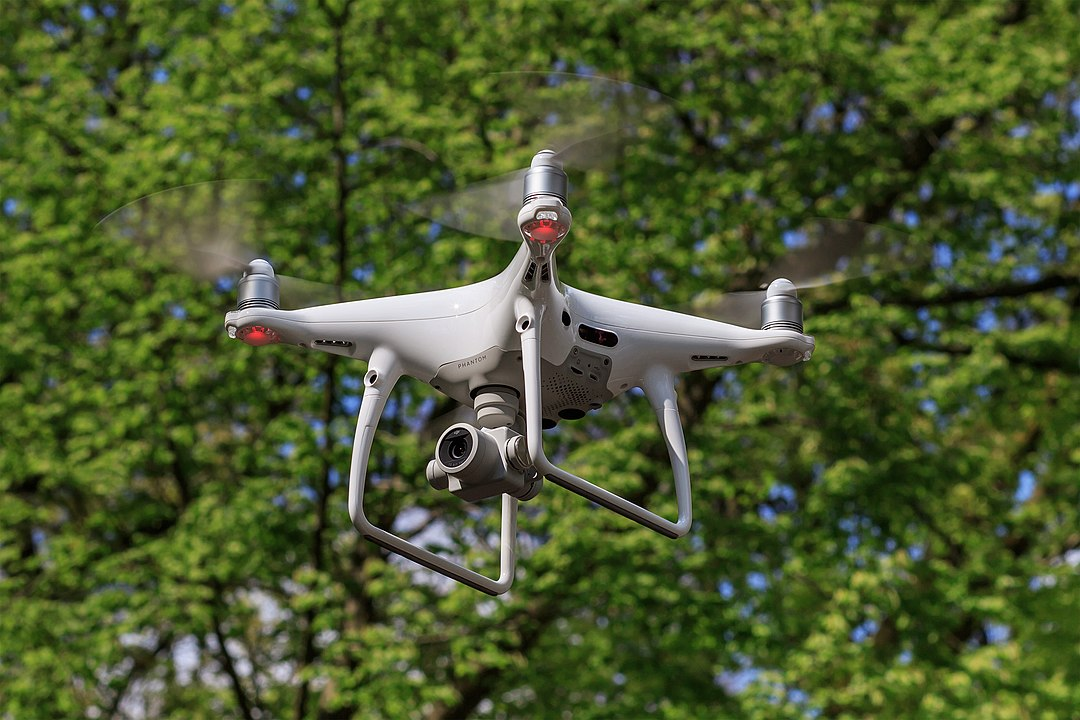
\includegraphics[scale=.08]{images/dji_phantom_fig2.jpg}\hspccc
				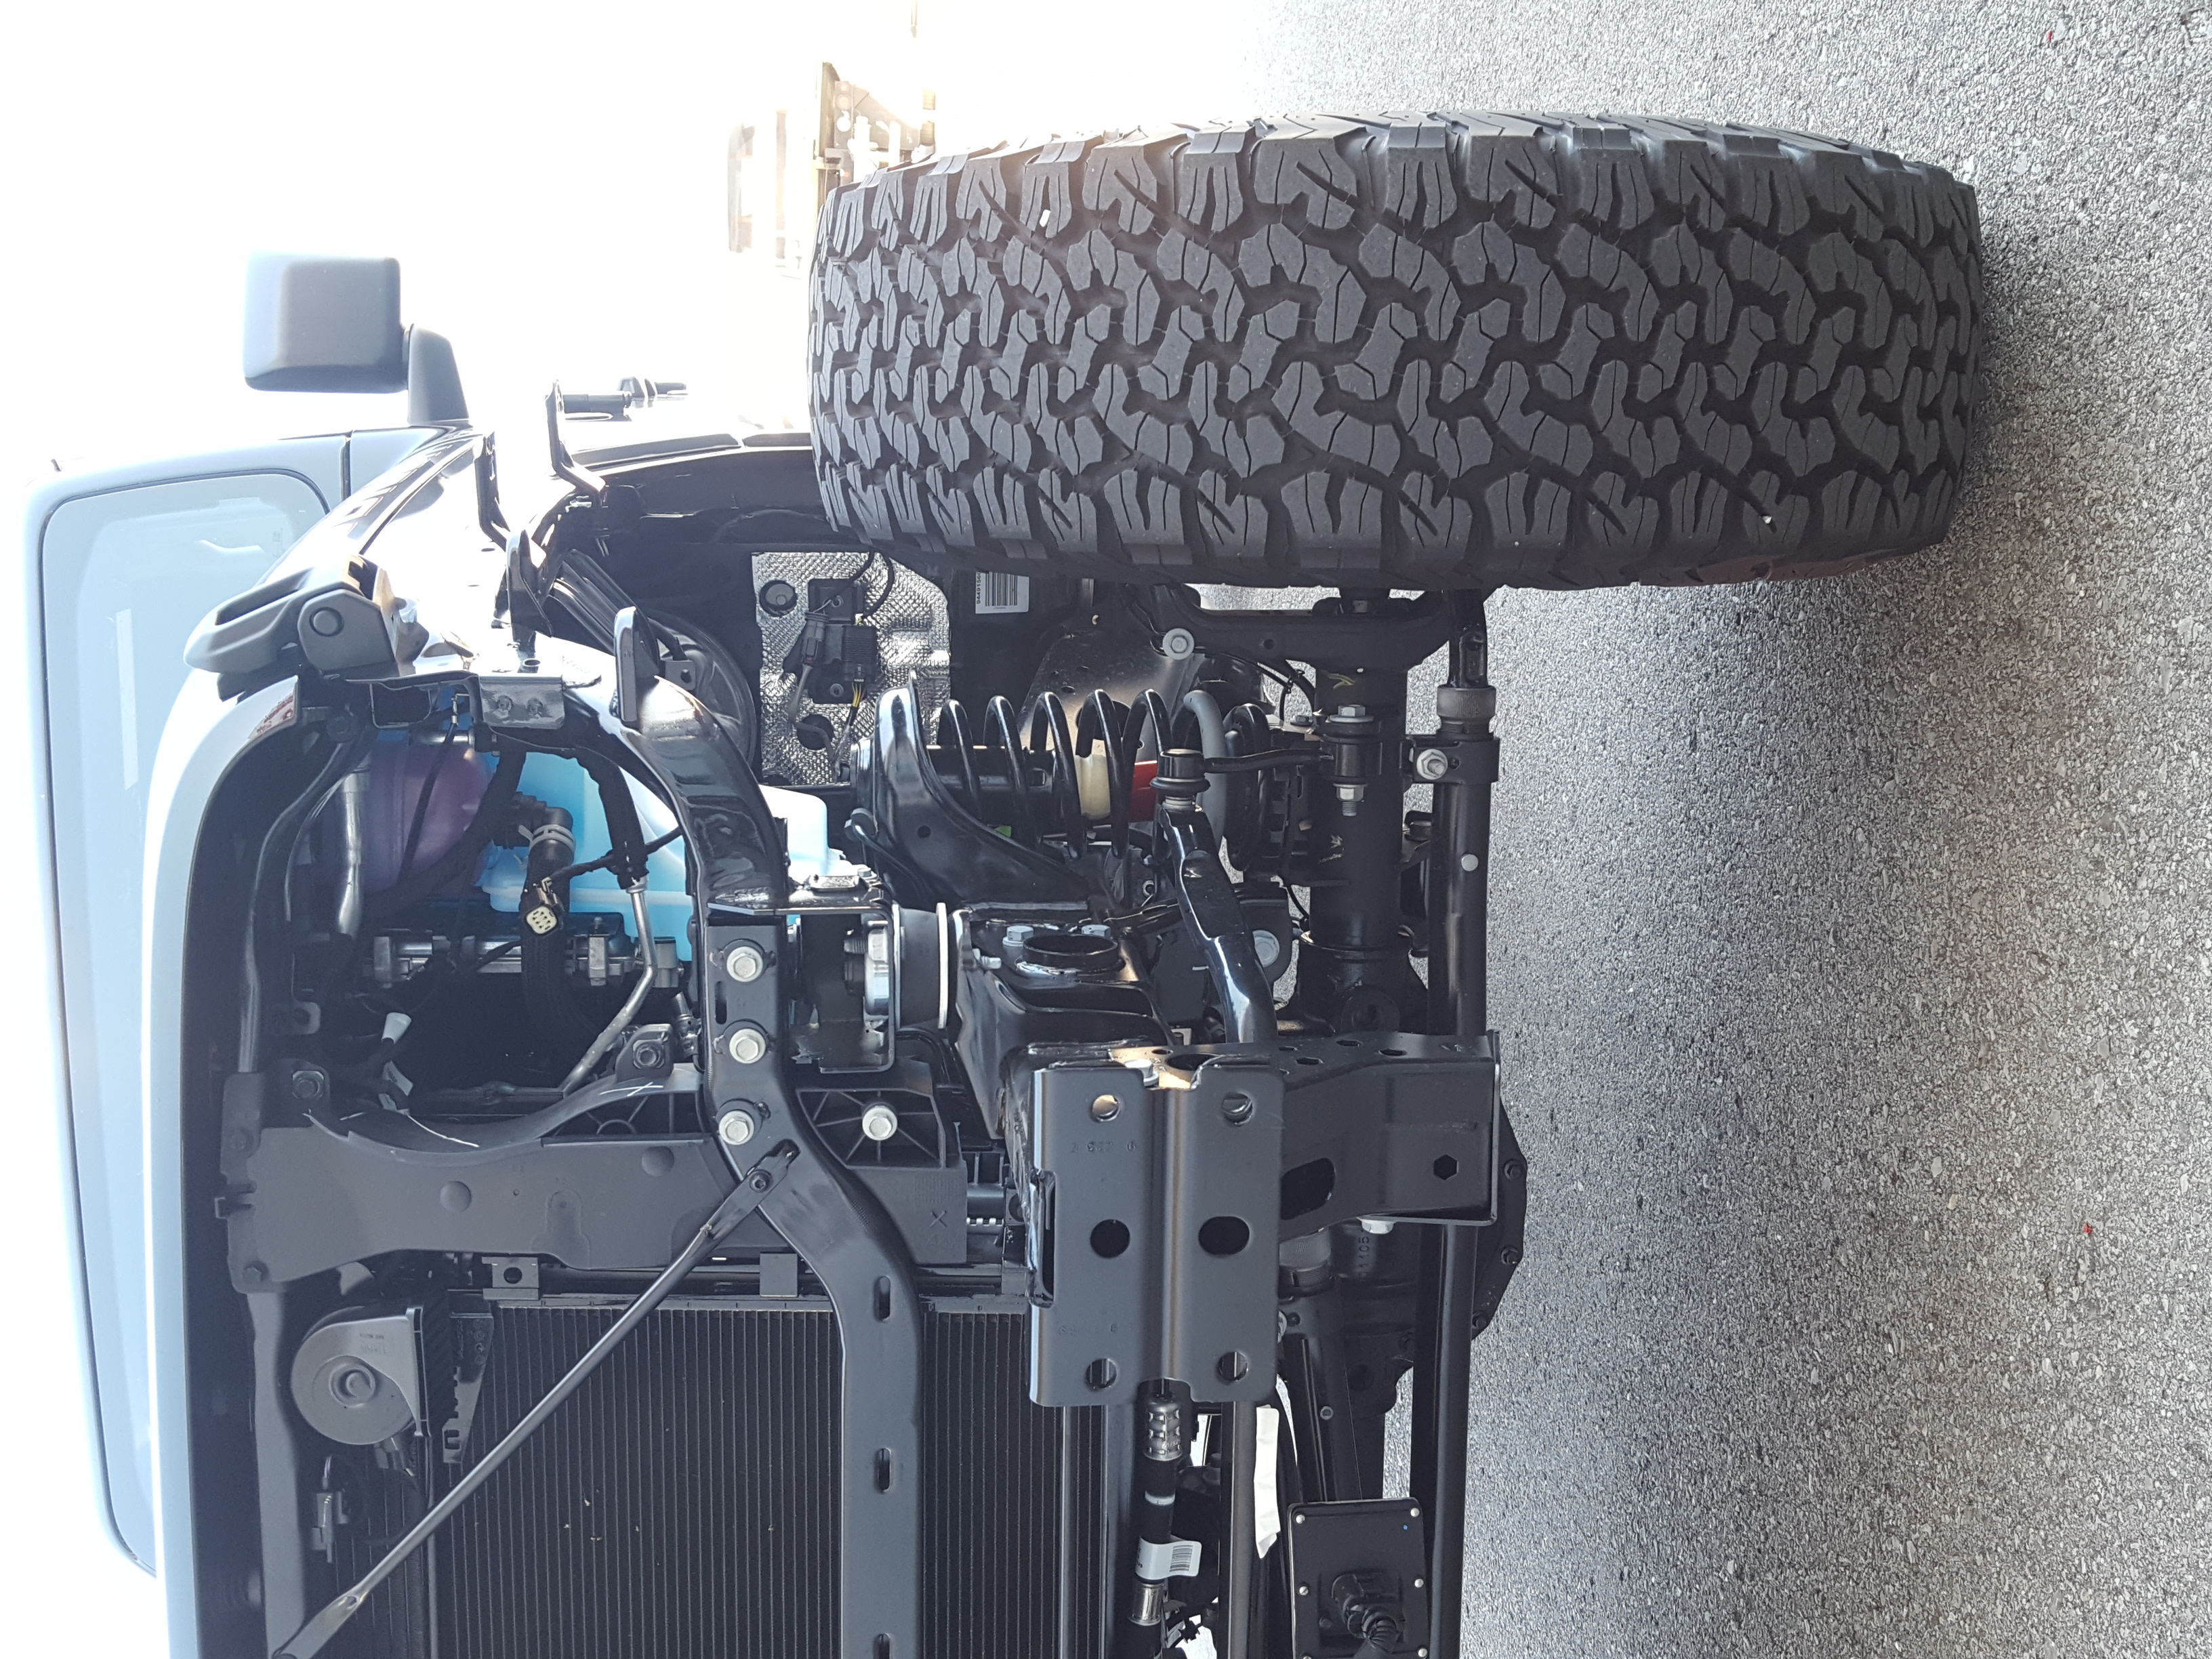
\includegraphics[scale=.025,angle=-90,origin=c]{images/jeep_01.jpg} \hspccc
				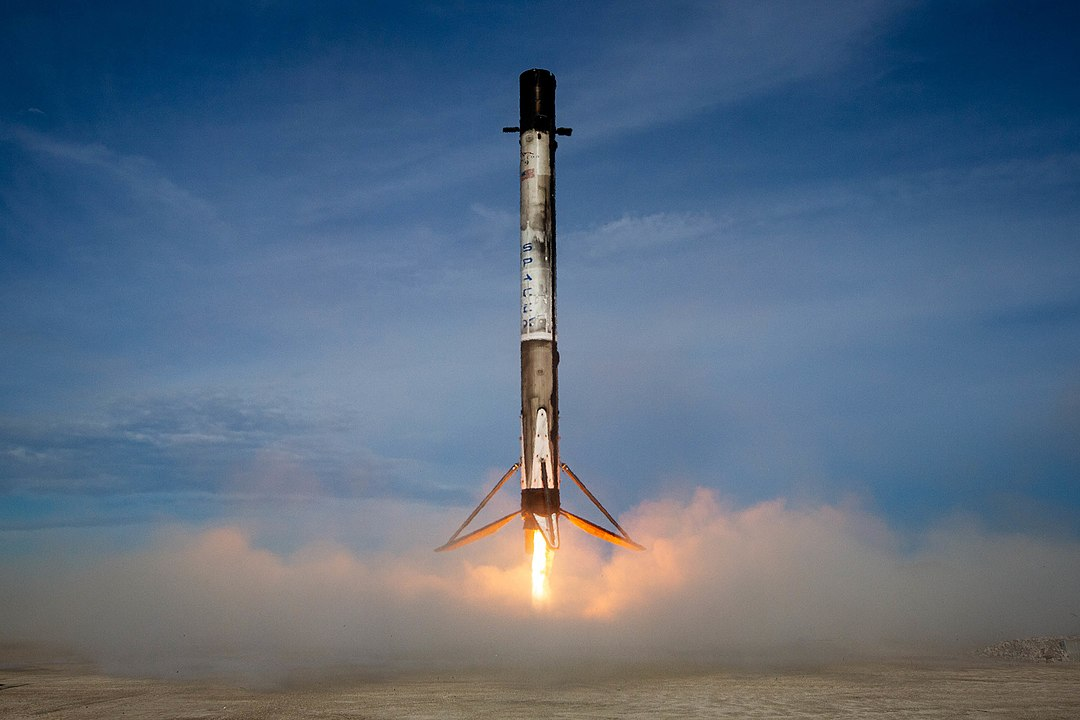
\includegraphics[scale=.1]{images/falcon9_fig2.jpg} \\
				{\tiny\href{https://en.wikipedia.org/wiki/Phantom_(UAV)}{Image: Wikipedia} \hspace{20mm}Image: TH \hspace{20mm}\href{https://en.wikipedia.org/wiki/SpaceX\#/media/File:CRS-18_Mission_(48380511427).jpg}{Image: Wikipedia} }

				\btVFill
			\end{frame}	

		% section I subsection IV
		\subsection{\sectionIsubsectionIVtitle}\label{sectionIsubsectionIV}	

			\begin{frame}
				\frametitle{\sectionIsubsectionIVtitle}
				\bigskip
				Discussion of ME3050 Course topics here

				\btVFill
			\end{frame}
	
	% Section II
	\section{\sectionIItitle}\label{sectionII}

		% section II Outline
		\begin{frame}
			\large \textbf{Topic 2 - \sectionIItitle} \vspace{3mm}\\

			\begin{itemize}
				\item \hyperlink{sectionIIsubsectionI}{\sectionIIsubsectionItitle} \vspc %  section II subsection I
				\item \hyperlink{sectionIIsubsectionII}{\sectionIIsubsectionIItitle} \vspc % section II subsection II
				\item \hyperlink{sectionIIsubsectionIII}{\sectionIIsubsectionIIItitle} \vspc % section II subsection III
				\item \hyperlink{sectionIIsubsectionIV}{\sectionIIsubsectionIVtitle} \vspc % section II subsection IV
			\end{itemize}

		\end{frame}

		% section II subsection I
		\subsection{\sectionIIsubsectionItitle}\label{sectionIIsubsectionI}

			\begin{frame}[label=sectionIIsubsectionI]
				\frametitle{\sectionIIsubsectionItitle}
				\bigskip
				
				\renewcommand{\arraystretch}{1.2}
				\begin{tabular}{|c|c|c|c|c|} \hline
				\textbf{Quantity}&\textbf{Unit(SI)} &\textbf{ Symbol(SI)}&\textbf{Unit(US)}&\textbf{Symbol(US)}\\ \hline
				time&second&(s)&second&(sec)\\ \hline
				length&meter&(m)&foot&(ft)\\ \hline
				force&newton&(N)&pound&(lb)\\ \hline
				mass&kilogram&(kg)&slug&(?) \\\hline
				energy&joule&(J)&foot-pound&(ft-lb)\\ \hline
				power&watt&(W)&?&(ft-lb/sec)\\ \hline
				temp.&degrees&$^\circ C$, $^\circ K$&degrees&$^\circ F$, $^\circ R$ \\ \hline
				\end{tabular}

				\vspace{3mm}When possible work in the {\it base} units. SI is preferred but engineers must know both systems.

				\btVFill
			\end{frame}

		    \begin{frame}[label=sectionIIsubsectionI]
				\frametitle{\sectionIIsubsectionItitle}
				\bigskip
				
				If you are unsure about the units, WRITE THEM OUT!

				Unit consistency is required for valid results. One method is to write out the conversion as a fraction and cancel the terms visually.\vspc

				\underline{Example}: Find the number of seconds that are in 3 days. \vspcc

				\scalebox{1.0}{$3$ Days $=$} 

				\btVFill
			\end{frame}	

		% section II subsection III
		\subsection{\sectionIIsubsectionIIItitle}\label{sectionIIsubsectionIII}

			\begin{frame}
				\frametitle{\sectionIIsubsectionIIItitle}
				\bigskip

				\begin{multicols}{2}

				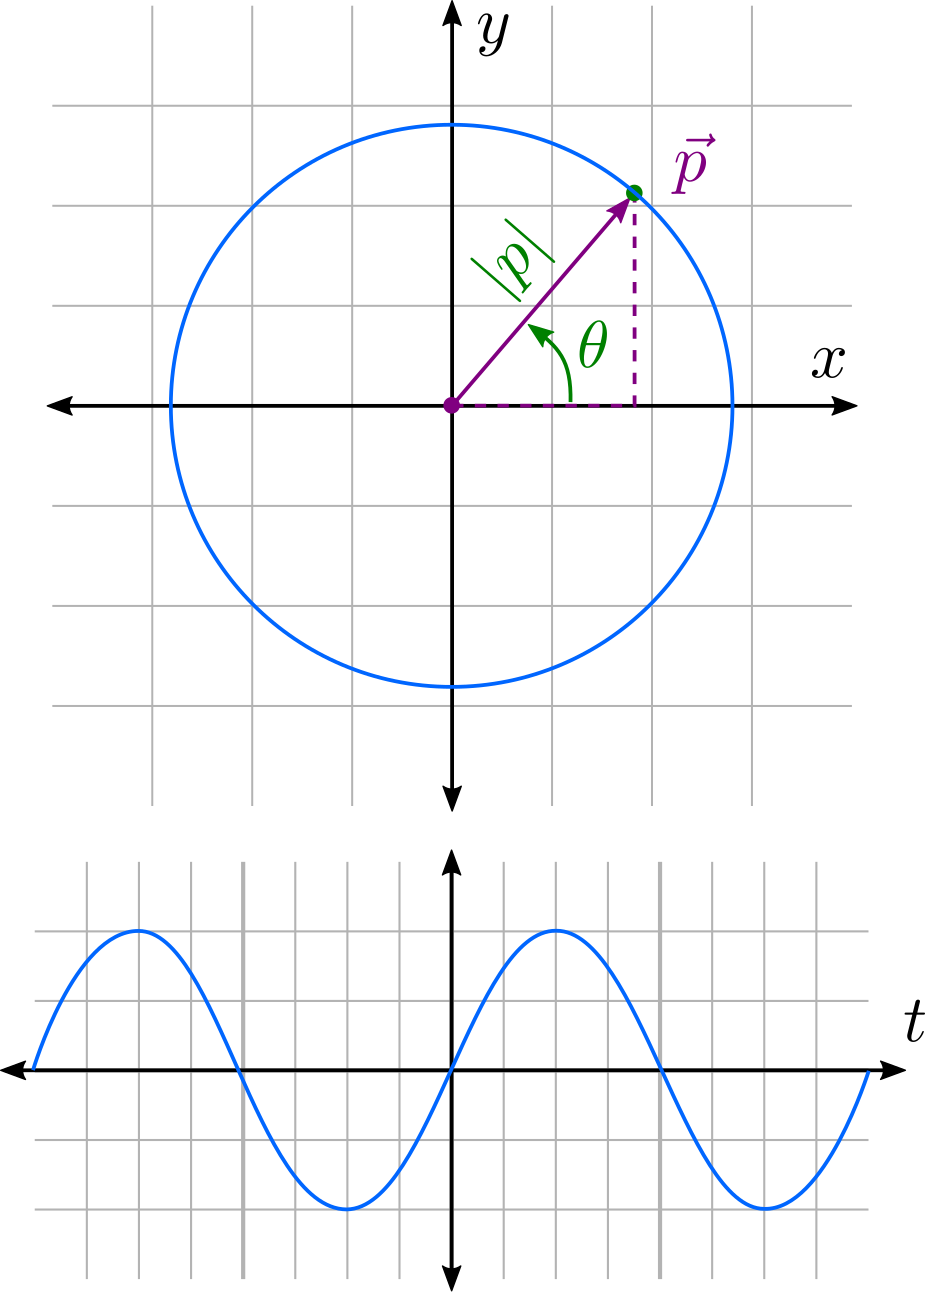
\includegraphics[scale=.16]{images/circular_frequency_fig2.png}

				Frequency ($Hz$) and circular-frequency ($\frac{rad}{s}$) are both commonly used. \vspace{15mm}

				You can easily convert from one to the other by multiplying or dividing by $2\pi$.
				\end{multicols}

				\btVFill {\tiny Image: TH}
			\end{frame}

		% section II subsection IV 
		\subsection{\sectionIIsubsectionIVtitle}\label{sectionIIsubsectionIV}

			\begin{frame}
				\frametitle{\sectionIIsubsectionIVtitle}
				\bigskip
				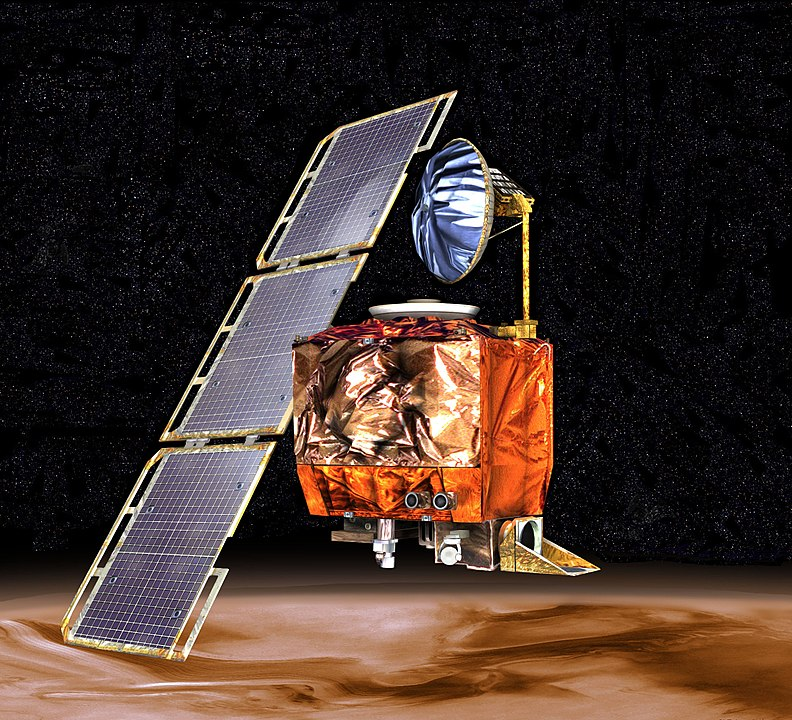
\includegraphics[scale=.1]{images/mars_orbiter.jpg}
				The Mars Climate Orbiter (formerly the Mars Surveyor '98 Orbiter) was a 638-kilogram (1,407 lb)[1] robotic space probe launched by NASA on December 11, 1998 to study the Martian climate, Martian atmosphere, and surface changes and to act as the communications relay in the Mars Surveyor '98 program for Mars Polar Lander. 
		
				\btVFill {\tiny \href{https://en.wikipedia.org/wiki/Mars_Climate_Orbiter}{Full Story and Images: Wikipedia} }
			\end{frame}
		
	% Section III
	\section{\sectionIIItitle}\label{sectionIII}

		% section III Outline
		\begin{frame}
			\large \textbf{Topic 3 - \sectionIIItitle} \vspace{3mm}\\

			\begin{itemize}
				\item \hyperlink{sectionIIIsubsectionI}{\sectionIIIsubsectionItitle} \vspc %  section III subsection I
				\item \hyperlink{sectionIIIsubsectionII}{\sectionIIIsubsectionIItitle} \vspc % section III subsection II
				\item \hyperlink{sectionIIIsubsectionIII}{\sectionIIIsubsectionIIItitle} \vspc % section III subsection III
				\item \hyperlink{sectionIIIsubsectionIV}{\sectionIIIsubsectionIVtitle} \vspc % section III subsection IV
			\end{itemize}

		\end{frame}

		% section III subsection I
		\subsection{\sectionIIIsubsectionItitle}\label{sectionIIIsubsectionI}

			\begin{frame}
				\frametitle{\sectionIIIsubsectionItitle}
				\bigskip
				\begin{multicols}{2}
				Engineers encounter complex systems and these systems are difficult to model and analyze.  Analysis requires multiple steps or processes and modeling requires iteration. Typically, you cannot solve these complex problems in your head alone. \vspc

				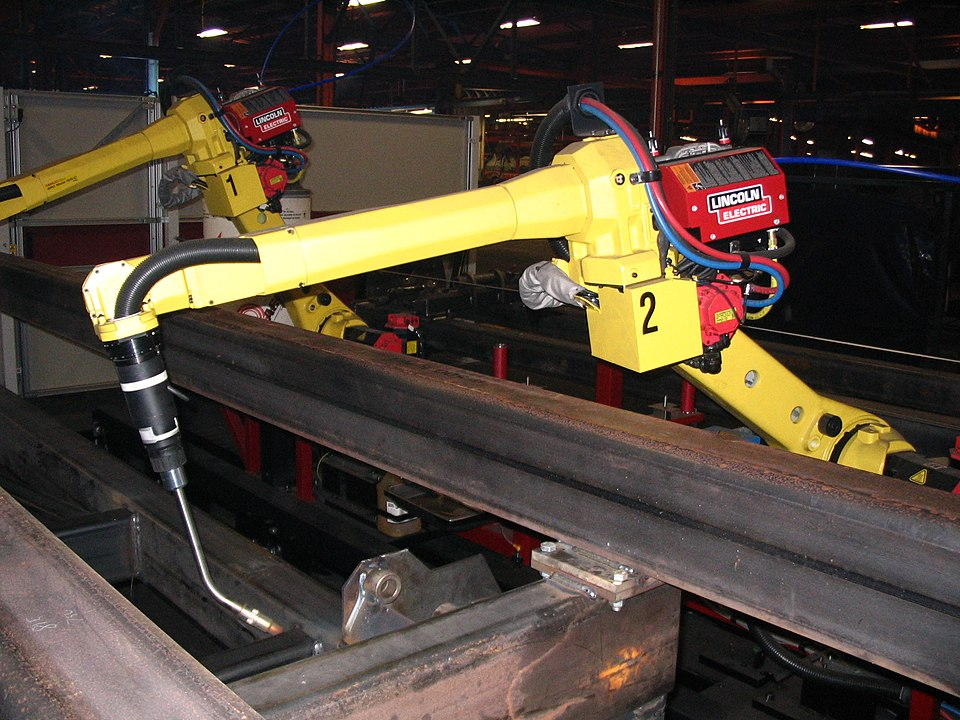
\includegraphics[scale=.15]{images/fanuc_robot.jpg}
				\end{multicols}
				{\tiny \hspace{60mm} Image: \href{https://en.wikipedia.org/wiki/Articulated_robot}{Wikipedia} }
		
				\btVFill
			\end{frame}

			\begin{frame}
				\frametitle{\sectionIIIsubsectionItitle}
				\bigskip
				Engineers model and analyze complex systems one piece at a time on a component level. \vspc

				In system dynamics we study the behavior of complex systems by modeling the iterations and responses of the different components involved. Our models will start simple and build in complexity as the theory is presented. 
	
				\btVFill
			\end{frame}

		% section III subsection II
		\subsection{\sectionIIIsubsectionIItitle}\label{sectionIIIsubsectionII}	

			\begin{frame}
				\frametitle{\sectionIIIsubsectionIItitle}
				\bigskip
				
				\begin{multicols}{2}
				\begin{itemize}
				\item Frictionless Sliding  ?
				\item Pure Roll - No Slip 
				\item Planar Motion \\
				\end{itemize}

				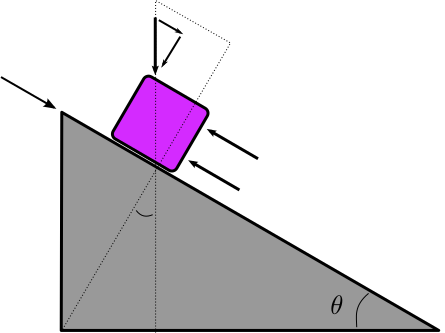
\includegraphics[scale=0.209]{images/sliding_block.png}
				 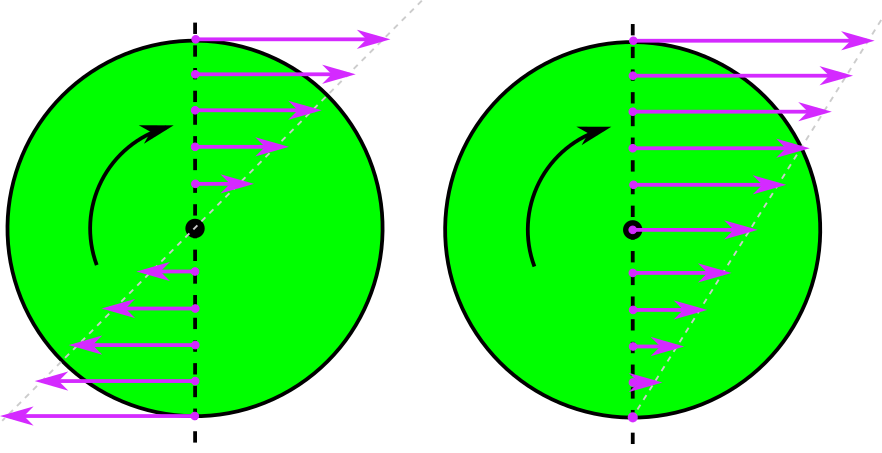
\includegraphics[scale=0.125]{images/pure_roll_no_slip.png} 
				 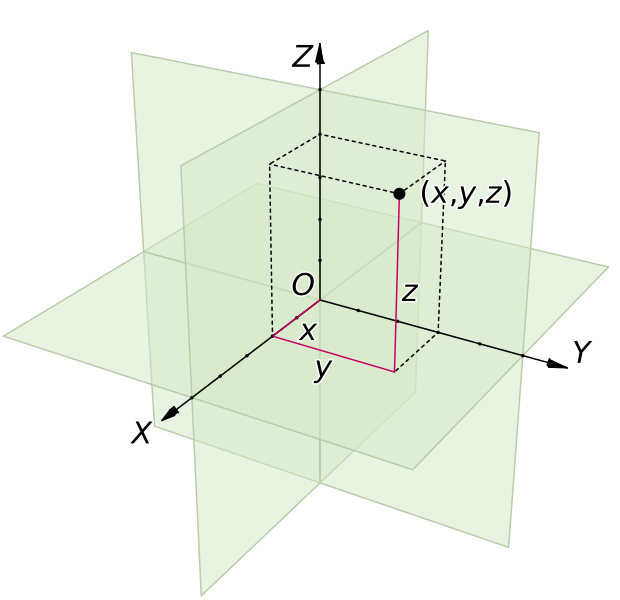
\includegraphics[scale=0.17]{images/cartesian_3d.png}
				\end{multicols}
				{\tiny Image: TH\hspace{60mm} Images: TH, \href{https://en.wikipedia.org/wiki/Cartesian_coordinate_system}{Wikipedia} }

				\btVFill
			\end{frame}

		% section III subsection III
		\subsection{\sectionIIIsubsectionIIItitle}\label{sectionIIIsubsectionIII}

			\begin{frame}
				\frametitle{\sectionIIIsubsectionIIItitle}
				\bigskip
				
				\begin{itemize}
					\item Viscous Boundary Layer
					\item Insulated or Constant Flux Boundaries
					\item Others?
				\end{itemize}	

				\btVFill
			\end{frame}

		% section III subsection IV
		\subsection{\sectionIIIsubsectionIVtitle}\label{sectionIIIsubsectionIV}	

			\begin{frame}
				\frametitle{\sectionIIIsubsectionIVtitle}
				%\bigskip
				\begin{multicols}{2}
					\begin{itemize}
					\item No Heat Loss or Generation
					\item Ideal Conductors
					\item Zero Order, First Order System Behavior
					\end{itemize}

					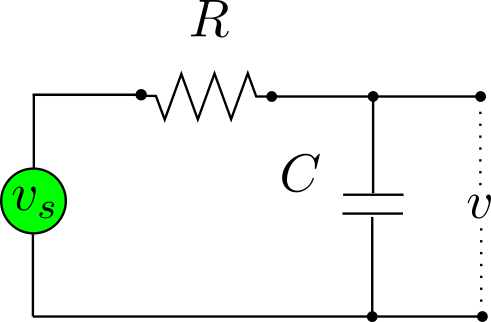
\includegraphics[scale=.25]{images/rc_circuit.png}
				\end{multicols}
				
				\btVFill {\tiny Image: TH}
			\end{frame}

\end{document}





